\subsection{Análise mensal}
Foi realizada uma análise mês a mês a fim de identificar, a partir de uma nova perspectiva. Para isso, foi gerada uma tabela com um resumo das médias dos tempos de espera, serviço e de chegada de ligação mês a mês.\\
A partir disso, foi possível calcular a porcentagem de falha (\%\_failure), com base na divisão do número total de ligações que demoraram mais de 60 segundos para serem atendidas pelo total de ligações atendidas em cada mês. 
A partir dessa tabela \ref*{fig: tmes}  é possível retirar algumas conclusões relevantes e transformar a base de dados com filtro mês a mês em informações capazes de nos demonstrar o comportamento do processo de atendimento nos quesitos tempo de espera médio, duração média do atendimento, média do tempo entre as chegadas, média do número de ligações recebidas e também a porcentagem de falhas.  
\begin{figure}[H]
    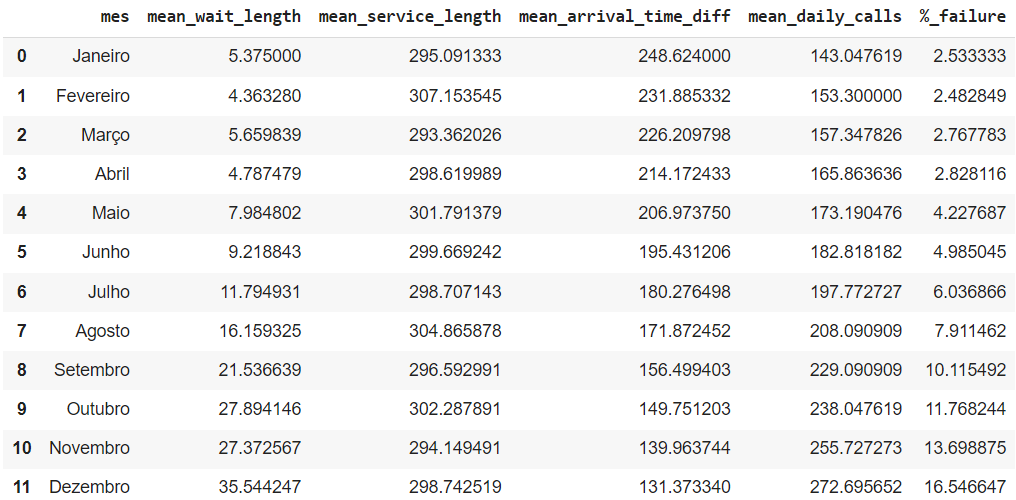
\includegraphics{analise-de-dados/mensal/tabmens.png}
    \caption{Tabela de resumo das médias dos tempos de espera, serviço e de chegada de ligações mês a mês}
    \label{fig: tmes}
\end{figure}

Realizando uma análise de cada uma das variáveis analisadas, é possível obter:
\begin{itemize}
    \item Tempo de espera: Aumenta mês a mês
    \item Média do tempo de serviço: Relativamente constantes
    \item Tempo entre chegadas: Diminui mensalmente
    \item Número de ligações: Aumenta mensalmente
    \item Percentual de falhas: Aumenta mês a mês. A partir de setembro de 2021, a tolerância de 10\% que foi estipulada pelo gerente é superada e, a partir desta data se mantêm assim.\\
Portanto, o percentual falhas, aqui definido como o percentual de chamadas que demoram mais de 60 segundos para serem atendidas, aumenta mês a mês, ultrapassando, a partir de setembro de 2021, a tolerância de 10\% estipulada pelo gerente e a operação começa a ficar fora das metas estipuladas pela gerência

